\chapter{How to Access Sora 2 and Veo 3}
\label{ch:accessing-sora2}

\begin{chapterabstract}
This chapter provides comprehensive guidance on accessing and configuring the two leading AI video generation platforms: OpenAI's Sora 2 and Google's Veo 3. For Sora 2, we examine three primary access methods: the web-based desktop interface for precise parameter control, the iOS mobile application for portable creation, and the API for enterprise integration. The chapter details Sora 2's evolutionary improvements, including the unified cross-modal generation engine, the Cameo insertion system, enhanced physics simulation, voice synchronization capabilities, and extended video duration support up to 90 seconds. For Veo 3, we cover two access pathways: direct integration through Google Gemini Advanced, and the professional Flow platform (\url{https://labs.google/flow}) offering granular control over model selection and generation parameters. Practical instructions cover account registration, subscription tier selection, workspace configuration, and interface navigation for both platforms. By understanding these technical foundations, readers will be prepared to leverage either platform's capabilities while making informed decisions that align with their creative objectives.
\end{chapterabstract}

Before you truly begin crafting Prompts and envisioning shots, you must first learn ``how to enter the world of Sora 2.'' The purpose of this chapter is to help you thoroughly understand this gateway---what it is, where it is, how to use it, and why it is completely different from traditional video creation.

\section{What is Sora 2: A Generative Revolution from Text to Dynamic Imagery}
\index{Sora 2!definition}
\index{text-to-video generation}

Sora 2 is OpenAI's second-generation text-to-video system released in 2025, representing a milestone leap in the field of AI vision. It not only inherits the first-generation Sora's Text-to-Video capabilities but also integrates multimodal features such as images, voice, dialogue, sound effects, and physical simulation, allowing creators to directly generate ``complete cinematic narratives'' through ``textual language.''

\subsection{Redefining ``Creation''}
\index{creative workflow!AI transformation}

In traditional film and television production, going from concept to finished product requires at least four stages: script, shooting, editing, and color grading. In Sora 2's workflow, all of this is compressed into a single text description. Creators only need to write Prompts in natural language, and Sora 2 will automatically complete:

\begin{itemize}
\item Scene construction (light and shadow, color temperature, texture, physical relationships)
\item Cinematographic language (push, pull, pan, tilt, depth of field control, motion trajectories)
\item Audio design (dialogue, ambient sound, music matching)
\item Emotional rendering (expressing through character expressions and lighting atmosphere)
\end{itemize}

\subsection{Differences from Sora 1}
\index{Sora!version comparison}

Compared to the first generation, Sora 2's innovations include:

\begin{enumerate}
\item \textbf{Unified Cross-Modal Generation Engine}: Sora 2 can generate complete videos with images, sound, and dialogue in one go, rather than stitching together multiple models.
\item \textbf{Cameo Insertion System}\index{Cameo system}: Supports recording personal 3D facial models and voice characteristics on iOS applications to ``star'' in generated videos.
\item \textbf{Real Physics Perception and Lighting Consistency}: The model understands laws such as ``gravity,'' ``fluids,'' and ``reflection,'' making scenes naturally physically logical.
\item \textbf{Voice Synchronization System}: Dialogue tone, rhythm, and character lip movements perfectly match, with adjustments based on cultural context.
\item \textbf{Extended Duration and Memory Capability}: Can generate up to 90-second clips (for pro users) while maintaining contextual continuity for ads, MVs, tutorials, and narrative films.
\end{enumerate}

Sora 2's goal is not to replace human directors, but to give more ordinary people ``director-level creative power.''

\section{Official Access Points and Platform Channels}
\index{access methods}
\index{platform channels}

Currently, Sora 2 provides three main access methods:

\begin{enumerate}
\item \textbf{Web Version (Desktop)}: Suitable for users who need precise control over shot parameters and export formats.
\item \textbf{iOS Application (Sora App for iPhone)}: Portable version, suitable for creating and previewing anytime, anywhere.
\item \textbf{API Interface (For Developers)}: Suitable for enterprises and research institutions for system integration.
\end{enumerate}

\subsection{Detailed Web Access Process}
\index{web access}

\begin{enumerate}
\item Open a recommended browser (latest versions of Chrome, Safari, or Edge).
\item Enter \texttt{https://sora.chatgpt.com/} in the address bar (or jump from the OpenAI official website).
\item The page displays buttons like ``Log in'' and ``Get Started''; click to enter.
\item If you already have a ChatGPT/OpenAI account, log in directly; otherwise, register and fill out an access application.
\item After successful login, you will see an interface containing the following modules:
\end{enumerate}

\begin{figure}[H]
\centering
\includegraphics[width=\textwidth]{Fig2-1.png}
\caption{Sora 2 web interface showing main control panels \\ \authorillustration}
\label{fig:ch02-web-interface}
\end{figure}

\begin{itemize}
\item \textbf{Prompt Input Box}: Enter your text description.
\item \textbf{Parameter Panel}: Configure video orientation (Portrait/Landscape) and duration (10s/15s) through intuitive toggle and dropdown controls.
\item \textbf{Preview Window}: Real-time display of generation progress and results.
\item \textbf{History Panel}: Saves each generation, supports reuse and variant generation.
\item \textbf{Export/Share Function}: One-click download of MP4 or share links to social media.
\end{itemize}

\begin{Prompt}
\textbf{Note}: If you see ``Waitlist'' or ``Invite Only'' after logging in, it means the current region is not yet fully open and requires an invitation code or waiting list placement.
\end{Prompt}

\subsection{iOS Version Installation and Usage}
\index{iOS app}

\begin{itemize}
\item Open the App Store and search for \textbf{``Sora by OpenAI''}.
\item If your region (such as the US, Japan, Canada) supports it, click install.
\item After launching, follow instructions to log in to your OpenAI account.
\item If prompted for an invitation code, enter the code from official or test invitation emails.
\item Some regions may trigger identity verification upon first login, such as recording a short video to verify cameo functionality.
\end{itemize}

\begin{Prompt}
According to Japanese media reports, the Sora 2 app can be downloaded directly, but core generation features are still limited by \textbf{invitation system}.
\end{Prompt}

\begin{figure}[H]
\centering
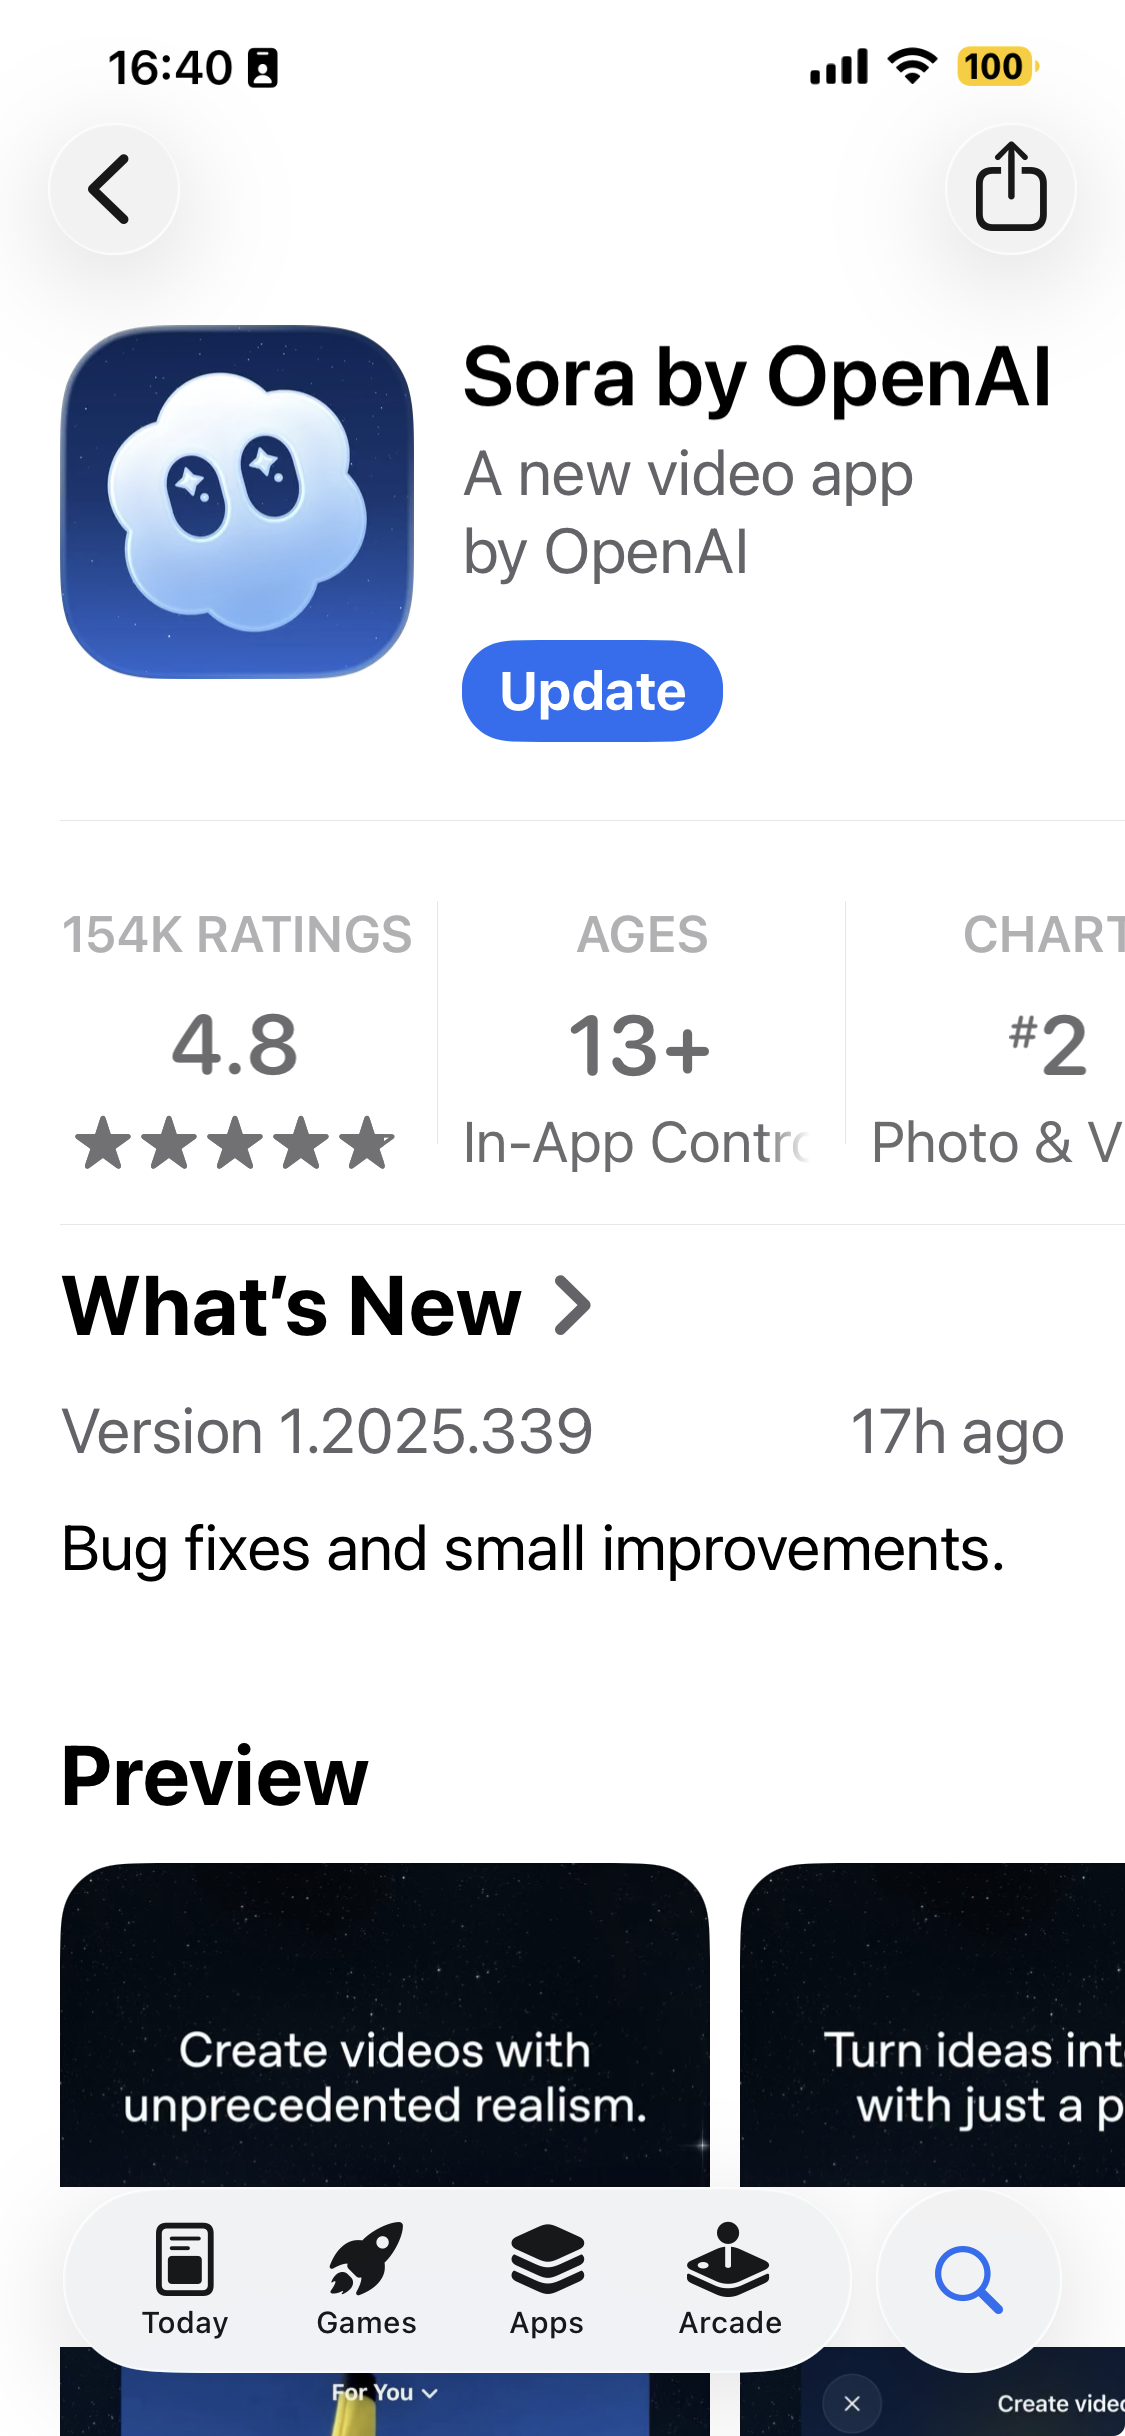
\includegraphics[height=\figheight]{Fig2-2.png}
\caption{Sora 2 app download page on iOS App Store \\ \authorillustration}
\label{fig:ch02-appstore-download}
\end{figure}

\subsection{Android Version}
\index{Android app}

As of October 2025, the Android version is in pre-registration phase. Users can pre-order on Google Play. After official launch, it will support the same functional modules and account system as iOS.

\section{Regional Differences and Access Permissions}
\index{regional availability}
\index{access restrictions}

OpenAI's opening strategy for Sora 2 adopts a ``regional phased'' model:

\begin{table}[H]
\centering
\caption{Regional Availability of Sora 2 \\ \authorillustration}
\label{tab:regional-access}
\begin{tabular}{|l|l|l|l|}
\hline
\textbf{Region} & \textbf{Status} & \textbf{Restrictions} & \textbf{Notes} \\
\hline
US / Canada & Open (Invite-only) & Requires invite code & Web \& iOS supported \\
Japan & Downloadable, partial lock & Cameo needs invite & Good localization \\
Europe & Partial pilot & GDPR review & Future compliance \\
China / HK / Taiwan & Not yet open & Can use overseas account & Requires stable VPN \\
\hline
\end{tabular}
\end{table}

This regional strategy reflects both technical deployment needs and policy, privacy protection, and server location considerations. OpenAI plans to deploy regional nodes in more countries to synchronously improve generation speed and access quality.

\section{Registration and Login: From Account System to Security Mechanisms}
\index{account system}
\index{security}

\subsection{OpenAI's Unified Account System}

Sora 2 shares the same login architecture with ChatGPT. Users with existing OpenAI accounts can use them directly without creating new ones. All generated content is bound to the ``Drafts'' page under that account for easy synchronization and backup.

\begin{figure}[H]
\centering
\includegraphics[height=\figheight]{Fig2-3.png}
\caption{Unified OpenAI account dashboard \\ \authorillustration}
\label{fig:ch02-account}
\end{figure}

\subsection{Invitation System and Qualification Mechanism}
\index{invitation system}

Based on OpenAI's official announcement on September 30, 2025, and subsequent release information, Sora 2 adopts a strict, phased invitation system for access.

Here is accurate information about Sora 2's invitation and access mechanisms (as of October 2025):

\subsubsection{Core Invitation Mechanism: Invitation Code System}

Sora 2 is currently not an open registration or pay-to-use product. It is in an early limited rollout phase, with invitation codes being the core access method.

\textbf{``1 Invites 4'' Model:}
This is currently the primary way to gain access. Each user officially approved to join receives 4 invitation codes, which they can share with others.

\subsubsection{Official Invitation Channels}

\textbf{iOS App Waitlist:}
Users can download Sora 2's standalone iOS application, log in with their OpenAI account, and click ``Notify me when access opens'' to join the official waitlist.

\textbf{Pro User Priority:}
OpenAI explicitly states that paid subscribers (such as ChatGPT Pro users) have higher priority on the waitlist and will receive invitations earlier.

\textbf{Geographic Restrictions:}
Sora 2's initial release is limited to the United States and Canada. Users from other countries and regions (including China) currently cannot access it through official channels and must wait for subsequent global rollout plans.

\subsubsection{Key Feature Access Mechanism (Cameo)}

Sora 2 introduces a powerful feature called ``Cameo'' that allows users to incorporate real people's (including themselves and friends) likenesses and voices into generated videos. Due to portrait rights and ethical risks, this feature has very strict access mechanisms:

\textbf{Personal Verification Required:}
Users cannot arbitrarily use others' likenesses.

\textbf{``Liveness Detection'':}
To create a ``Cameo,'' users must record a 5-15 second verification video within the app. The system Prompts users to complete specific actions (such as turning their head or saying specific phrases) to prove voluntary participation and that they are real people (not photos or recordings).

\textbf{Permission Control:}
Even after users create their own Cameo, they can finely control its usage, such as setting it to ``self-use only,'' ``specific friends only,'' or ``public.''

\subsubsection{Internal Qualification Review and Security Mechanisms}

Beyond user-side invitation systems, Sora 2 has strict internal review mechanisms to prevent abuse:

\textbf{Prompt Review:}
The system real-time scans user input Prompts, automatically blocking requests to generate violence, pornography, hate speech, or unauthorized public figures.

\textbf{Content Traceability:}
All videos generated by Sora 2 are mandatorily embedded with visible dynamic watermarks and invisible C2PA metadata to clearly identify them as AI-generated.

\textbf{Multi-layer Scanning:}
Even if Prompts pass review, the system performs ``frame-by-frame scanning'' after video rendering to detect hidden violating content.



\subsection{Login Security and Privacy Protection}
\index{privacy protection}
\index{two-factor authentication}

\begin{itemize}
\item Enable two-factor authentication (2FA) recommended.
\item Cameo uploads require authorization confirmation to avoid portrait and copyright disputes.
\item System encrypts and stores generation history, allowing users to delete all data records.
\end{itemize}

\section{Initial Interface Explanation and Usage Tips}
\index{user interface}

Based on the actual Sora WebUI interface, the platform adopts a social media-style design similar to TikTok, optimized for mobile-first video creation and sharing. The interface consists of several key areas:

\subsection{Main Feed Interface}
\index{main feed}

The primary interface displays a vertical video feed with the following elements:

\begin{enumerate}
\item \textbf{Video Display Area}:
\begin{itemize}
\item Vertical video thumbnails arranged in a grid layout
\item Each video shows a preview frame with the Sora watermark
\item Videos display engagement metrics: likes, comments, views, and shares
\item Creator usernames are prominently displayed below each video
\end{itemize}

\item \textbf{Navigation Tabs}:
\begin{itemize}
\item ``For you'' tab for personalized content discovery
\item Left sidebar with navigation icons for different sections
\item Clean, minimalist design focusing on content consumption
\end{itemize}
\end{enumerate}

\subsection{Video Creation Interface}
\index{video creation}

The creation interface is accessed through the bottom input area:

\begin{enumerate}
\item \textbf{Prompt Input}:
\begin{itemize}
\item ``Describe your video...'' text input field at the bottom
\item Simple, conversational Prompt interface
\item ``+'' button to upload reference images
\end{itemize}

\item \textbf{Generation Parameters}:
\begin{itemize}
\item \textbf{Orientation}: Toggle between Portrait and Landscape modes
\item \textbf{Duration}: Selectable options including 10 seconds, 15 seconds
\item Parameters appear as overlay options during creation
\end{itemize}
\end{enumerate}

\subsection{Activity and Notifications Panel}
\index{activity panel}

The Activity panel provides real-time updates on your creations:

\begin{enumerate}
\item \textbf{Generation Status}:
\begin{itemize}
\item ``Your draft is ready'' notifications
\item ``Your video generation failed'' error messages
\item Real-time progress updates with thumbnail previews
\end{itemize}

\item \textbf{Organization}:
\begin{itemize}
\item ``New'' section for recent activities
\item ``All'' section for complete history
\item Each notification includes Prompt preview and generation status
\end{itemize}
\end{enumerate}

\subsection{User Profile and Management}
\index{user profile}

The user profile section includes comprehensive account management:

\begin{enumerate}
\item \textbf{Profile Statistics}:
\begin{itemize}
\item Followers count
\item Cameos count (for personalized avatar features)
\item Likes and Remixes received
\item Profile customization options (``Add bio'', profile picture)
\end{itemize}

\item \textbf{Content Organization}:
\begin{itemize}
\item \textbf{Posts}: Your published videos
\item \textbf{Cameos}: Personalized avatar creations
\item \textbf{Likes}: Videos you've liked
\item ``Drafts'' section for work-in-progress content
\end{itemize}

\item \textbf{Sharing and Collaboration}:
\begin{itemize}
\item ``Share'' button for profile sharing
\item ``Edit cameo'' for avatar customization
\item Social features integrated throughout the platform
\end{itemize}
\end{enumerate}

\subsection{Key Interface Design Principles}

\begin{itemize}
\item \textbf{Mobile-First Design}: Optimized for touch interaction and vertical viewing
\item \textbf{Social Integration}: Built-in sharing, following, and engagement features
\item \textbf{Simplified Creation}: Minimal barriers between idea and video generation
\item \textbf{Real-Time Feedback}: Immediate status updates and progress notifications
\item \textbf{Content Discovery}: Algorithm-driven feed for inspiration and community engagement
\end{itemize}

\subsection{Practical Usage Tips}

\begin{itemize}
\item \textbf{Prompt Writing}: Use clear, descriptive language in the ``Describe your video...'' field
\item \textbf{Parameter Selection}: Choose orientation based on intended platform (Portrait for mobile, Landscape for desktop)
\item \textbf{Duration Planning}: Start with shorter durations (10s) for faster generation and testing
\item \textbf{Activity Monitoring}: Regularly check the Activity panel for generation status and error messages
\item \textbf{Profile Management}: Organize content using the Posts/Cameos/Likes structure for easy retrieval
\end{itemize}

\section{Network and Access Optimization Strategies}
\index{network optimization}

Since generation involves large data transfers, network stability is key. Recommendations:

\begin{enumerate}
\item Use high-speed broadband or enterprise-grade Wi-Fi
\item If in restricted regions, use international network accelerators, but comply with local laws
\item Disable browser plugins to avoid script conflicts
\item Generate no more than two videos at a time to prevent system overload
\item Regularly clear cache to maintain page performance
\end{enumerate}

\section{Common Issues and In-Depth Solutions}
\index{troubleshooting}

\begin{table}[H]
\centering
\caption{Common Issues and Solutions \\ \authorillustration}
\label{tab:troubleshooting}
\small
\begin{tabular}{|p{3cm}|p{4cm}|p{5cm}|}
\hline
\textbf{Issue} & \textbf{Cause} & \textbf{Suggested Solution} \\
\hline
Login stuck loading & Invite code not activated or region restricted & Re-verify email, confirm IP region \\
\hline
Video stuttering or loading failure & Network delay or GPU queue & Lower resolution, shorten duration \\
\hline
Audio delay & Model not fully synchronized & Can correct in external software after generation \\
\hline
Cannot save video & Permission restriction or storage full & Clear history or upgrade account \\
\hline
\end{tabular}
\end{table}

\begin{Prompt}
\textbf{Tip}: If encountering ``Server Busy,'' try generating during off-peak hours (typically 2-5 AM US Pacific Time, when server load is lowest).
\end{Prompt}

\section{Ecosystem Extension: From Sora to the Creative Universe}
\index{ecosystem}
\index{future applications}

Sora 2 is not just a tool, but a hub for the future content industry. Its ecosystem will gradually expand in the following directions:

\begin{itemize}
\item \textbf{Education Sector}: Teachers can quickly create classroom demonstration videos
\item \textbf{Advertising Industry}: Brands can directly generate finished products from text scripts
\item \textbf{Filmmaking}: Directors use Sora 2 to quickly preview scenes or storyboards
\item \textbf{Social Platforms}: Creator communities can share Prompts and generated videos, realizing ``AI creative socialization''
\end{itemize}

Additionally, future support will include:

\begin{itemize}
\item \textbf{ChatGPT Integration}: Complete full-process video creation through natural conversational commands
\item \textbf{DALL·E and Voice Engine Linkage}: Form complete creation chain
\item \textbf{Enterprise API Services}: Provide customized model access for film, advertising, and educational enterprises
\end{itemize}

\section{Conclusion: Your Starting Point with Sora 2}
\index{getting started}

To smoothly enter the world of Sora 2, prepare the following:

\begin{enumerate}
\item A well-performing device (16GB RAM or more recommended)
\item Stable and secure international network
\item A valid OpenAI account and invitation code
\item Basic understanding of Prompt writing logic
\item Creative passion---this is a more important activation key than technology
\end{enumerate}

Once you complete login, understand the interface, and master basic commands, you will have the qualifications to ``enter the Sora universe.'' In the following chapters, we will delve into how to construct light, shadow, and emotion through text, making every Prompt you write a script-worthy directorial work.

\section*{Setup Templates}
\index{setup templates}

\subsection*{Template 1: Optimal Browser Configuration}
\begin{Prompt}
\textbf{Chrome/Safari Settings for Sora 2}:
\begin{itemize}
\item Enable Hardware Acceleration: Settings → Advanced → System
\item Increase Memory Allocation: chrome://flags → Memory Saver (Disabled)
\item Clear Cache: Developer Tools → Application → Storage → Clear Site Data
\item Disable Extensions: Temporarily disable ad blockers and privacy tools for https://sora.chatgpt.com/
\end{itemize}
\end{Prompt}



\subsection*{Template 3: Quality Control Workflow}
\begin{Prompt}
\textbf{Generation → Review → Iterate → Export Process}:
\begin{enumerate}
\item Generate initial version with basic Prompt
\item Review for technical quality (resolution, artifacts, consistency)
\item Iterate with refined Prompts based on initial results
\item Export final version in appropriate format for intended use
\item Document successful Prompt patterns for future reference
\end{enumerate}
\end{Prompt}

\section*{Troubleshooting Checklist}
\index{troubleshooting}

\subsection*{Common Access Issues}
\begin{itemize}
\item[$\square$] \textbf{Login Problems}: Verify OpenAI account status and subscription tier
\item[$\square$] \textbf{Slow Loading}: Check network connection and try different server regions
\item[$\square$] \textbf{Generation Failures}: Ensure Prompt doesn't violate content policies
\item[$\square$] \textbf{Export Issues}: Verify sufficient local storage space (2GB+ recommended)
\item[$\square$] \textbf{Quality Problems}: Adjust generation settings and retry with simplified Prompts
\end{itemize}

\subsection*{Performance Optimization}
\begin{itemize}
\item[$\square$] \textbf{Memory Management}: Close unnecessary browser tabs and applications
\item[$\square$] \textbf{Network Stability}: Use wired connection when possible, avoid peak hours
\item[$\square$] \textbf{Device Temperature}: Ensure adequate cooling during extended sessions
\item[$\square$] \textbf{Browser Updates}: Keep browser updated to latest version for compatibility
\item[$\square$] \textbf{Cache Management}: Regularly clear browser cache to prevent conflicts
\end{itemize}

\section*{First Generation Workflow}
\index{first generation}

\begin{table}[H]
\centering
\caption{Step-by-Step First Generation Guide \\ \authorillustration}
\label{tab:first-generation}
\begin{tabular}{p{2cm}p{5cm}p{6cm}}
\hline
\textbf{Step} & \textbf{Action} & \textbf{Expected Result} \\
\hline
1. Login & Access https://sora.chatgpt.com/ with credentials & Dashboard loads with creation interface \\
\hline
2. Create & Input Prompt text OR select Cameo OR upload reference image & Content appears in creation area \\
\hline
3. Generate & Click generate button & Short video creation begins \\
\hline
\end{tabular}
\end{table}

\section{How to Access Google Veo 3}
\label{sec:accessing-veo3}
\index{Veo 3!access methods}
\index{Google!Veo 3}

While the majority of this book focuses on Sora 2, Google's Veo 3 (specifically Veo 3.1) represents a powerful alternative that excels in certain areas, particularly native audio generation and photorealistic rendering. This section provides comprehensive guidance on accessing Veo 3 through its two primary channels.

\subsection{Method 1: Direct Access via Google Gemini}
\index{Gemini!Veo 3 integration}

The most straightforward official channel for accessing Veo 3 is through Google's Gemini interface. This method typically requires a Gemini Advanced subscription or relevant testing permissions.

\textbf{Step-by-Step Access Process:}

\begin{enumerate}
\item \textbf{Open Gemini Interface}: Navigate to Gemini's web interface at \url{https://gemini.google.com/}
\item \textbf{Access Tools Menu}: Click the ``+'' button or ``Tools'' option located to the left of the input field
\item \textbf{Select Video Creation}: In the dropdown menu, select ``Create videos (Veo 3.1)''
\item \textbf{Enter Your Prompt}: Type your video description in the text field and submit
\end{enumerate}

\begin{figure}[H]
\centering
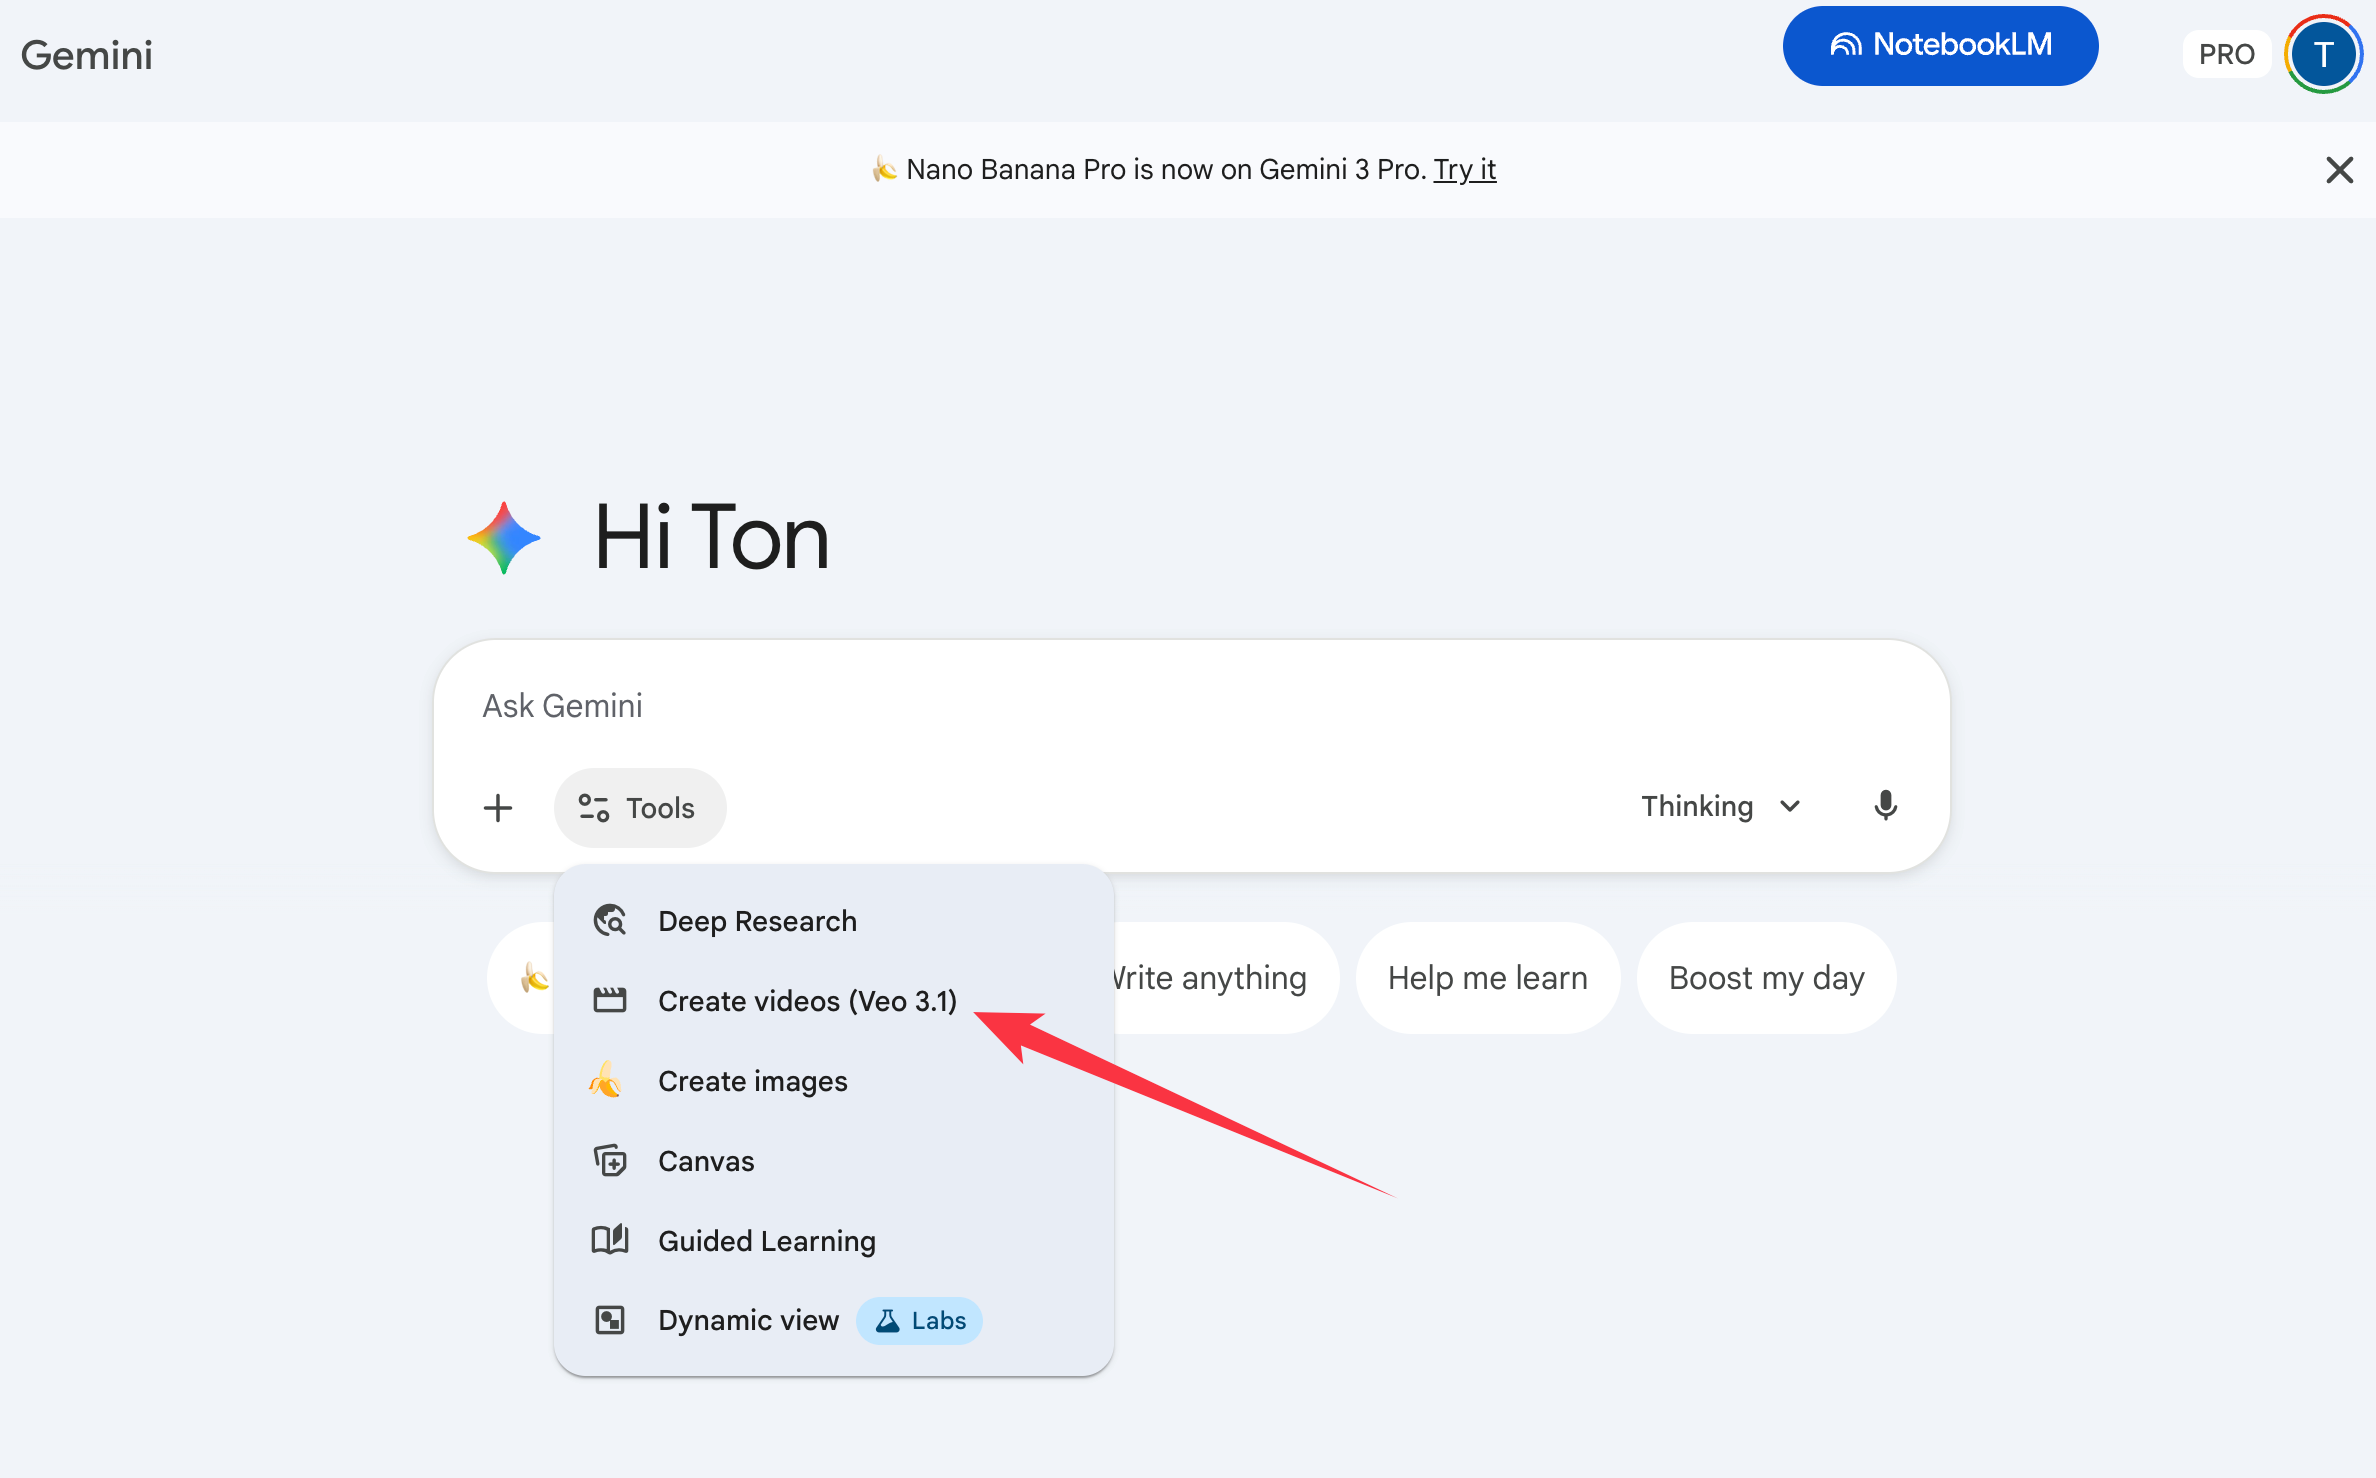
\includegraphics[height=\figheight]{Fig2-4.png}
\caption{Google Gemini interface showing the Tools menu with ``Create videos (Veo 3.1)'' option highlighted. This conversational interface provides the most accessible entry point for Veo 3 video generation. \\ \authorillustration}
\label{fig:gemini-veo3-tools}
\index{figure!Gemini Veo 3 interface}
\end{figure}

\begin{Prompt}
\textbf{Gemini + Veo 3.1 Quick Start}:
\begin{itemize}
\item Subscription: Gemini Advanced (\$19.99/month as of October 2025)
\item Interface: Conversational, similar to ChatGPT
\item Best For: Quick experiments, simple Prompts, beginners
\item Limitation: Less granular control over generation parameters
\end{itemize}
\end{Prompt}

\subsection{Method 2: Professional Access via Google Flow}
\index{Google Flow}
\index{Scenebuilder}

For creators requiring more precise control over video generation parameters, Google's Flow platform (\url{https://labs.google/flow}) provides a professional-grade interface with the ``Scenebuilder'' tool.

\textbf{Key Features of Flow/Scenebuilder:}

\begin{itemize}
\item \textbf{Multiple Generation Modes}:
  \begin{itemize}
  \item Text-to-Video: Generate videos from text Prompts
  \item Frame-to-Video: Animate static images or keyframes
  \item Asset-to-Video: Transform existing media assets
  \end{itemize}

\item \textbf{Model Selection}: Choose between different Veo versions:
  \begin{itemize}
  \item \textbf{Veo 3.1 - Fast} (Beta Audio): Faster generation with audio synthesis
  \item \textbf{Veo 3.1 - Quality} (Beta Audio): Higher visual quality with audio
  \item \textbf{Veo 2 - Fast}: Legacy version without audio
  \item \textbf{Veo 2 - Quality}: Legacy high-quality version without audio
  \end{itemize}

\item \textbf{Aspect Ratio Control}: Configure output dimensions (landscape, portrait, square)

\item \textbf{Credit System}: Each generation consumes credits (approximately 20 credits per generation with current settings)
\end{itemize}

\textbf{Step-by-Step Flow Access:}

\begin{enumerate}
\item \textbf{Navigate to Flow}: Visit \url{https://labs.google/flow}
\item \textbf{Sign In}: Use your Google account with appropriate permissions
\item \textbf{Select Generation Mode}: Choose ``Text-to-Video'' from the floating menu
\item \textbf{Configure Model}: Click the settings button above the input field to select your preferred Veo version
\item \textbf{Set Parameters}: Adjust aspect ratio and other settings as needed
\item \textbf{Generate}: Enter your Prompt and click the generate button
\end{enumerate}

\begin{figure}[H]
\centering
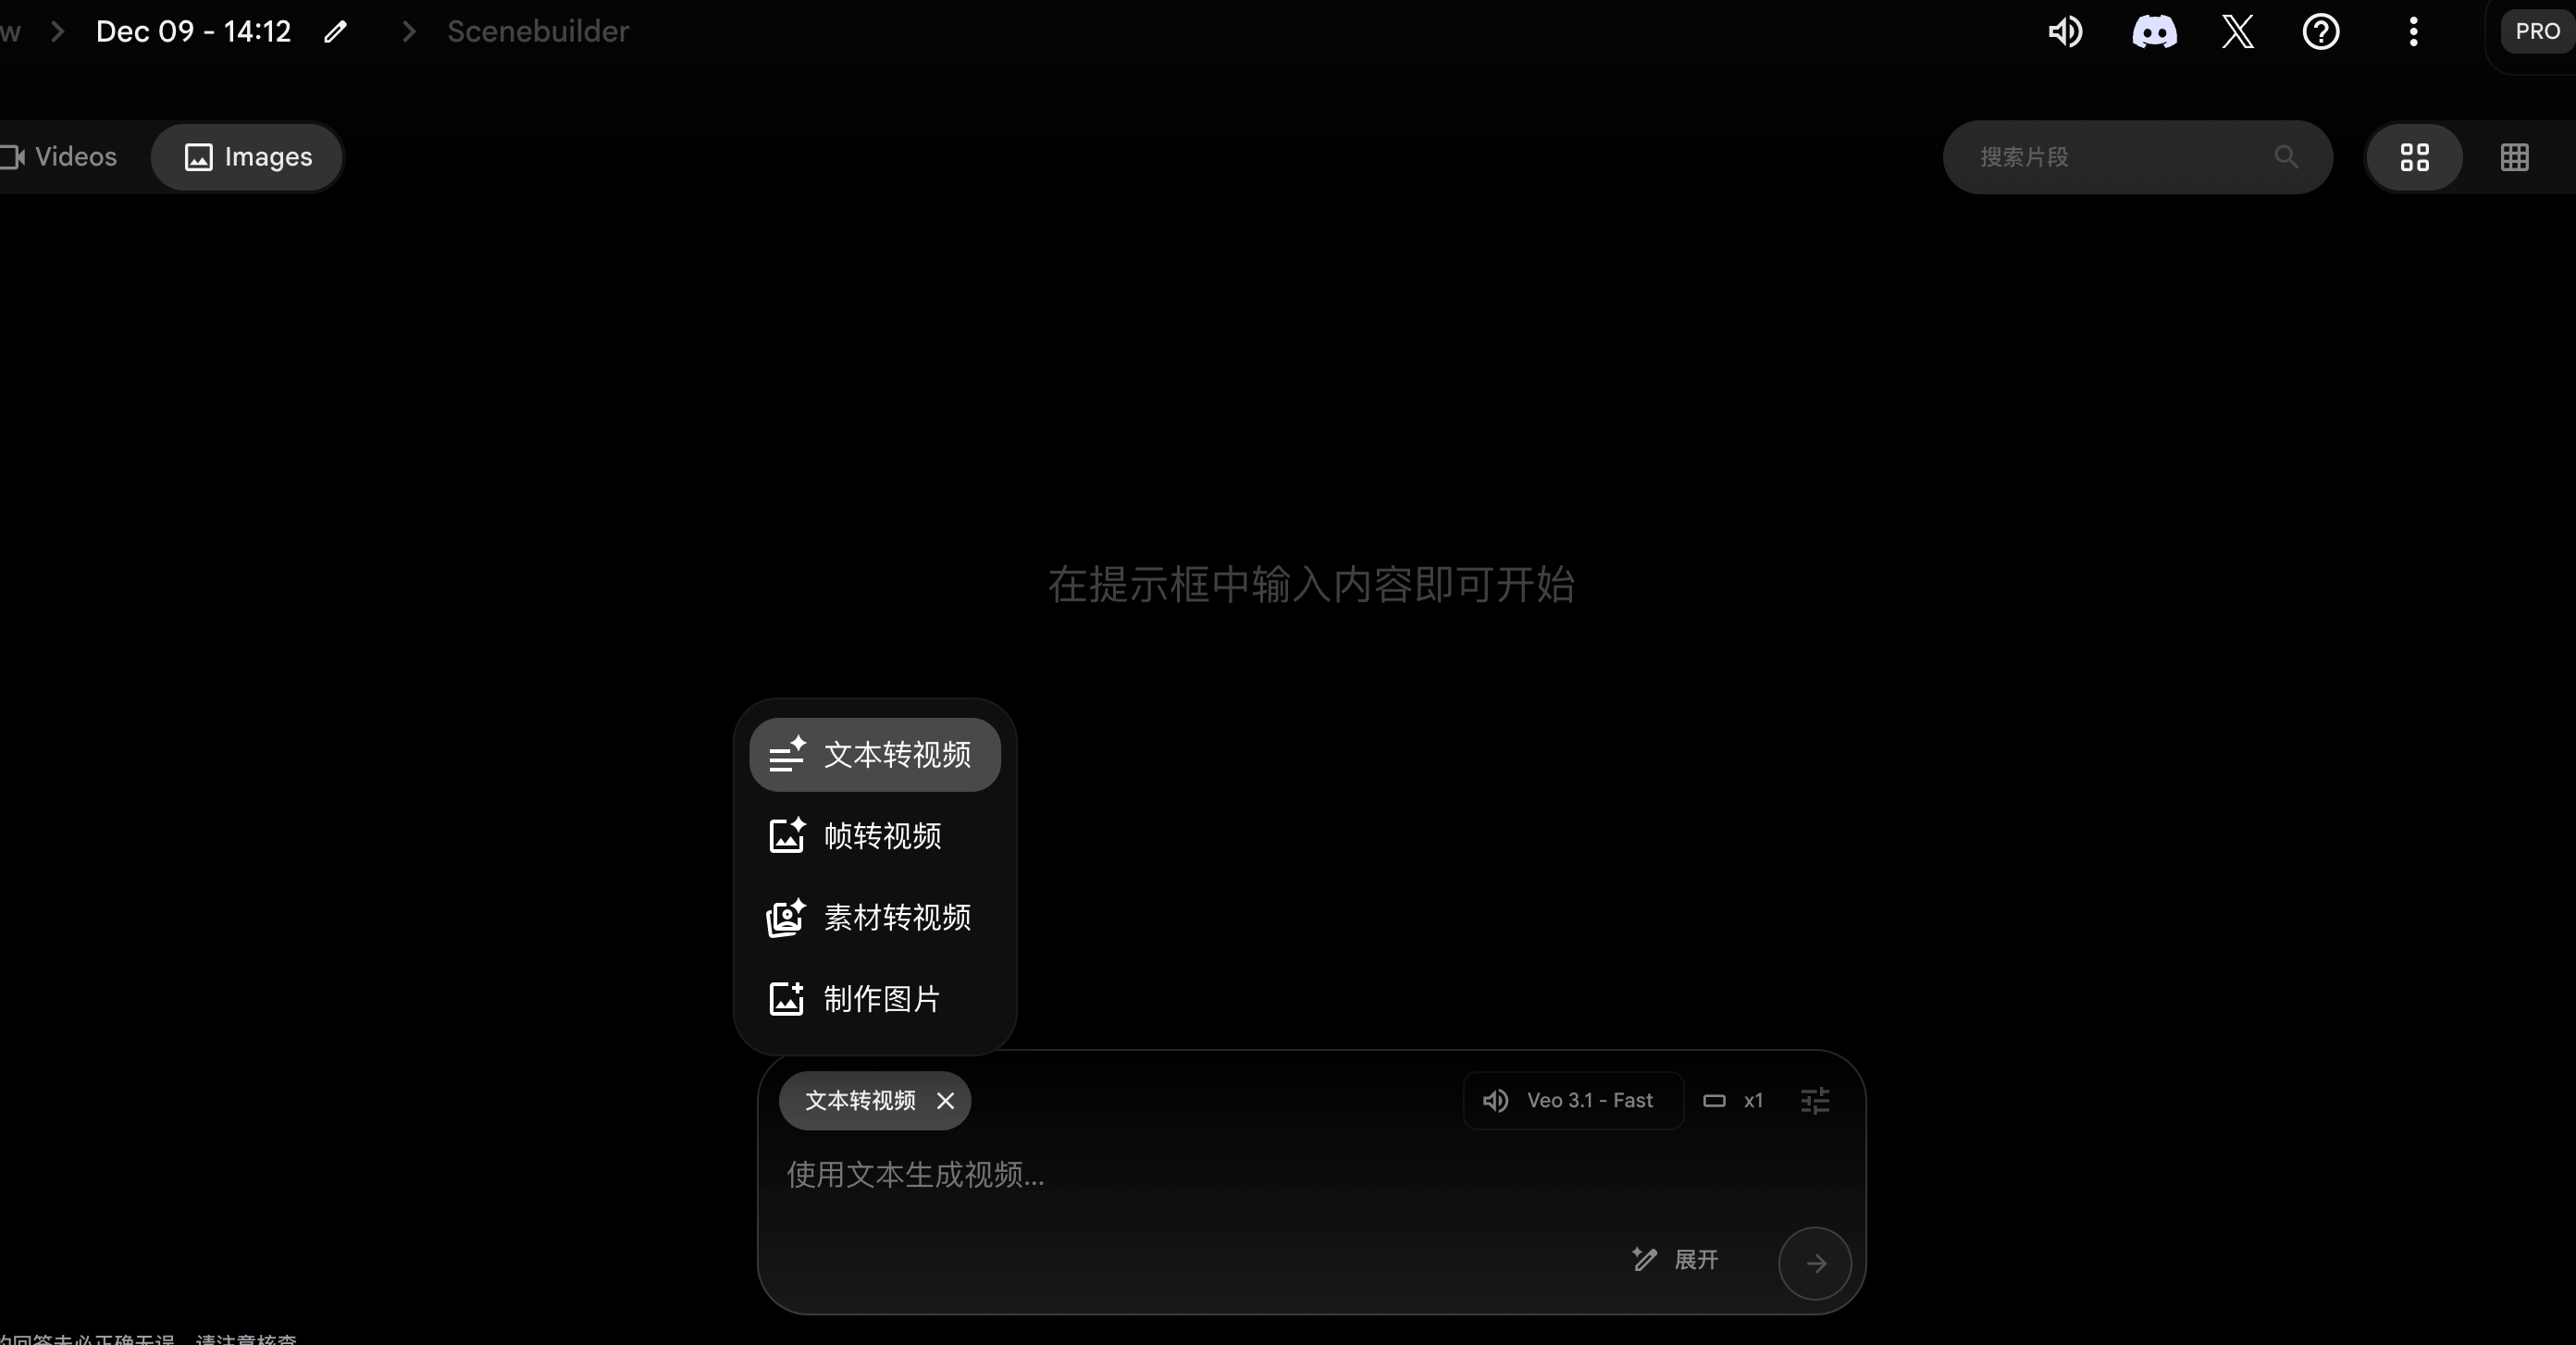
\includegraphics[height=\figheight]{Fig2-5.png}
\caption{Google Flow's Scenebuilder interface showing the main workspace. The floating menu on the left provides access to different generation modes including Text-to-Video, Frame-to-Video, and Asset-to-Video options. \\ \authorillustration}
\label{fig:flow-scenebuilder-main}
\index{figure!Flow Scenebuilder interface}
\end{figure}

\begin{figure}[H]
\centering
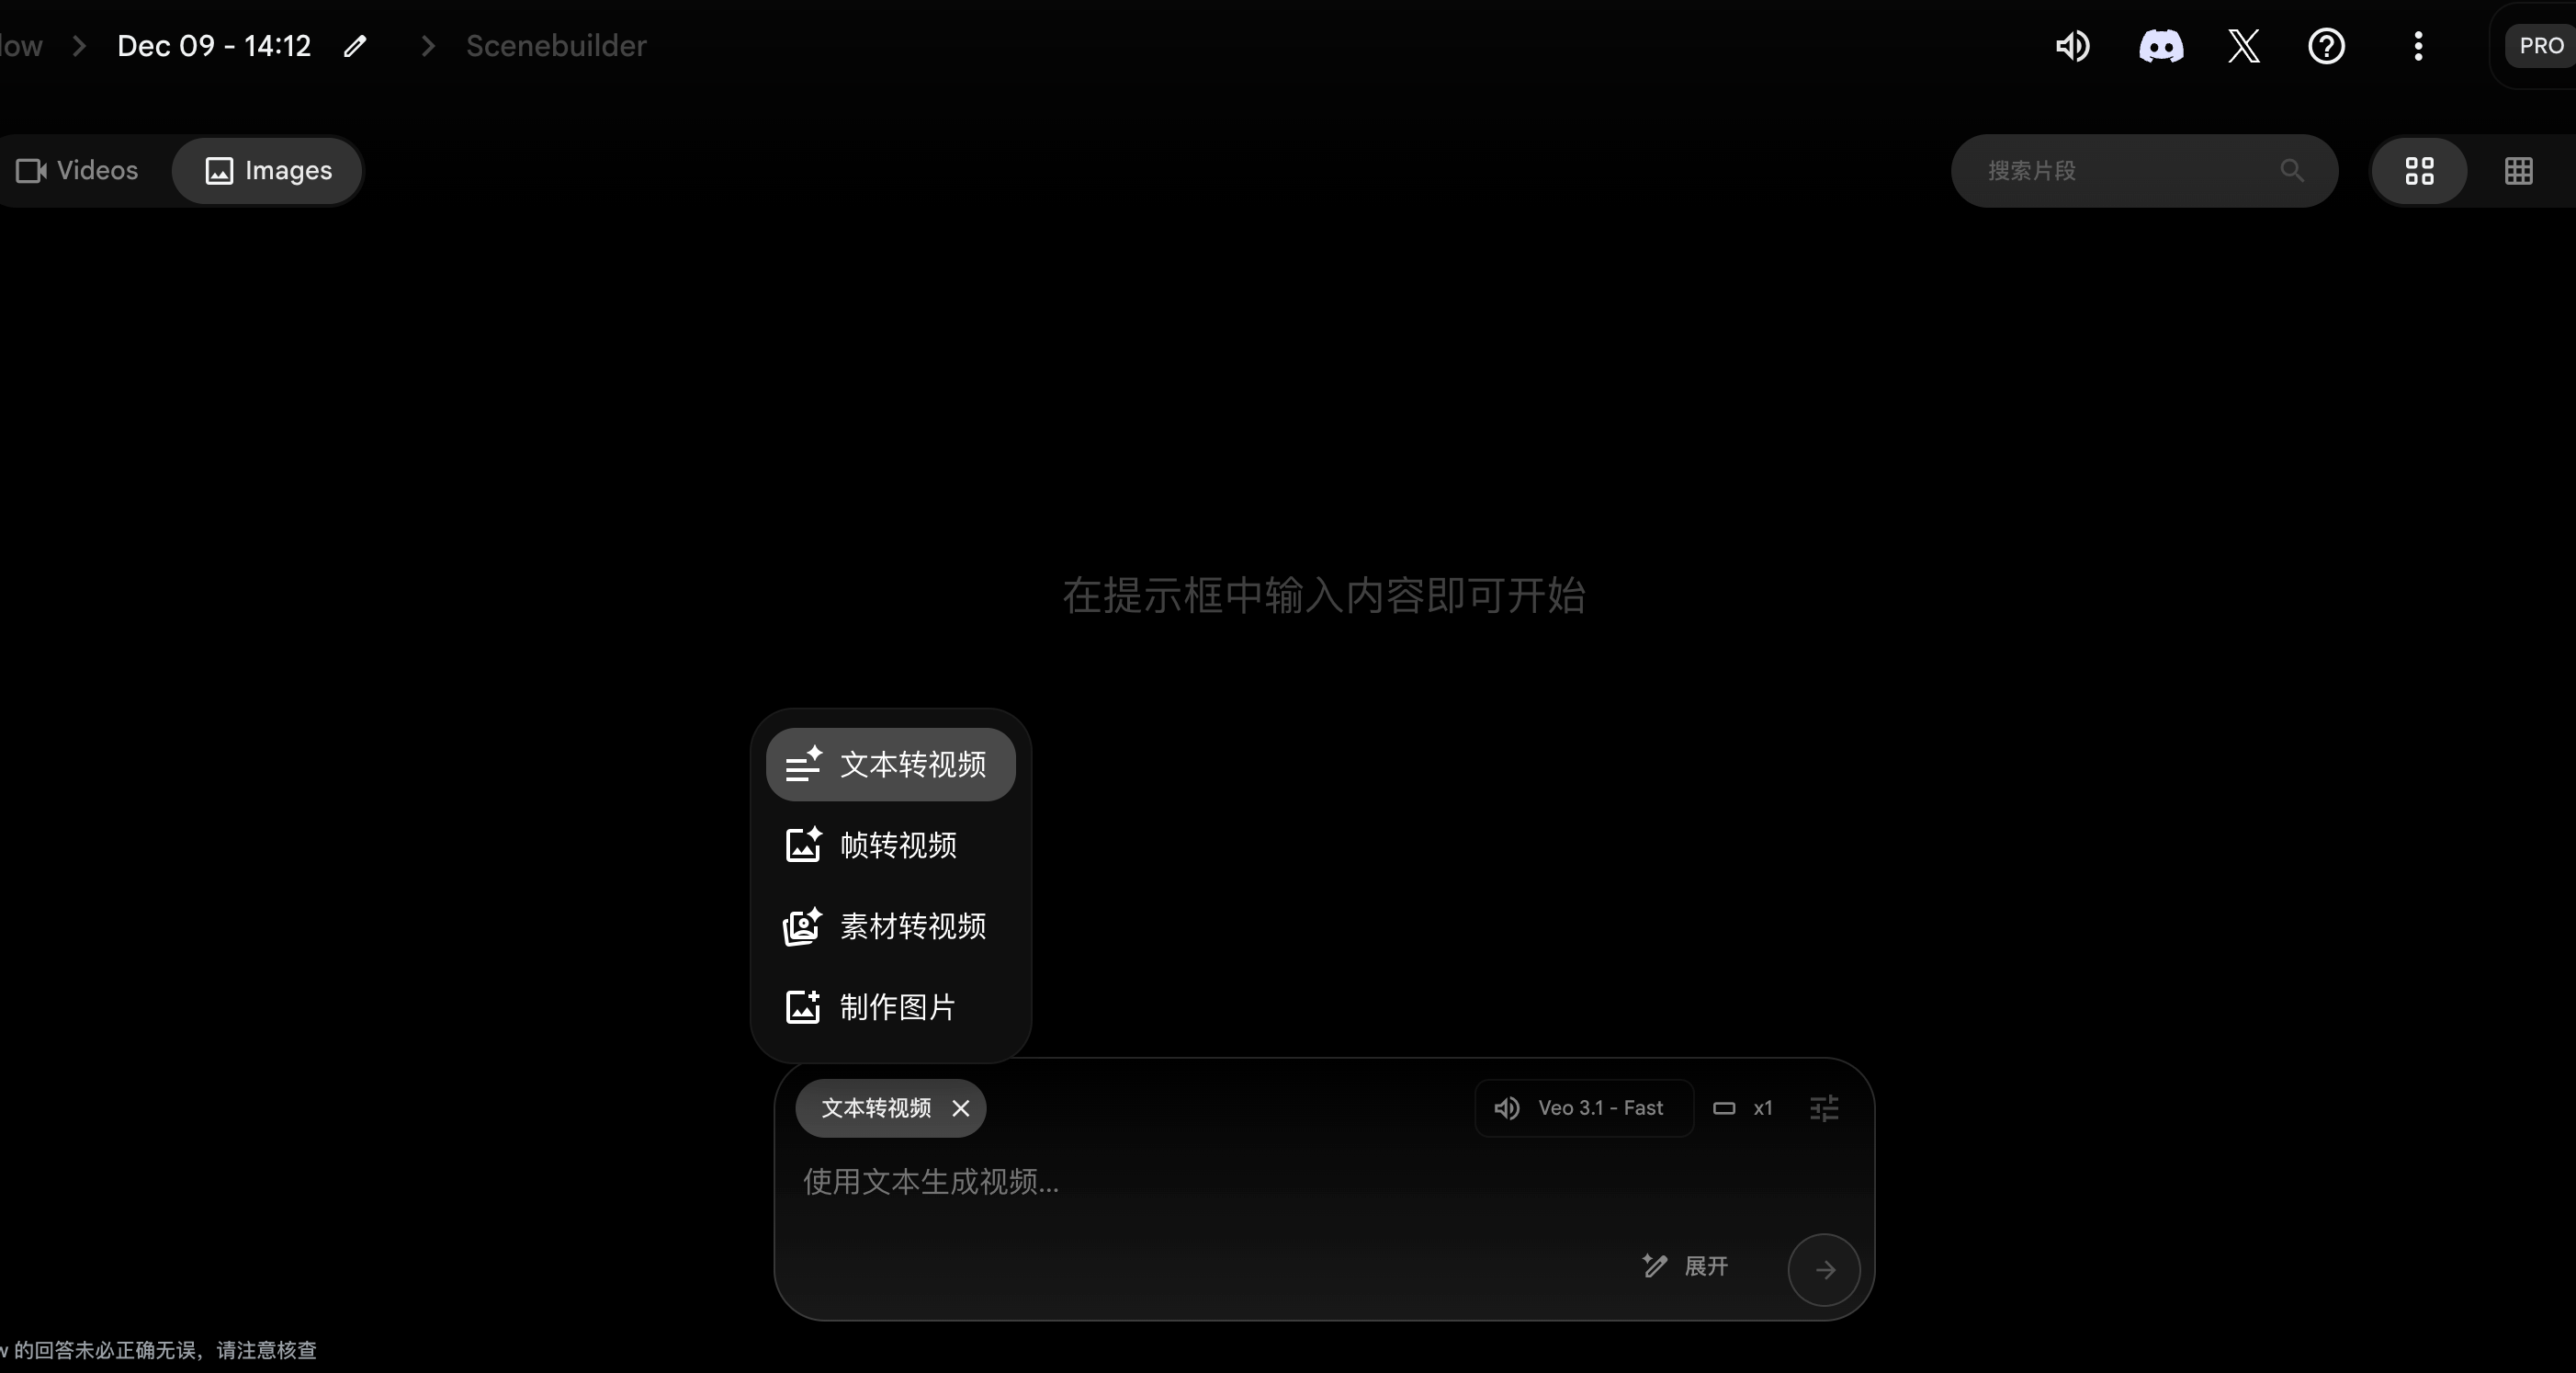
\includegraphics[height=\figheight]{Fig2-6.png}
\caption{Flow generation mode selection menu displaying Text-to-Video as the primary option. The interface also shows additional capabilities for frame-based and asset-based video generation workflows. \\ \authorillustration}
\label{fig:flow-generation-modes}
\index{figure!Flow generation modes}
\end{figure}

\begin{figure}[H]
\centering
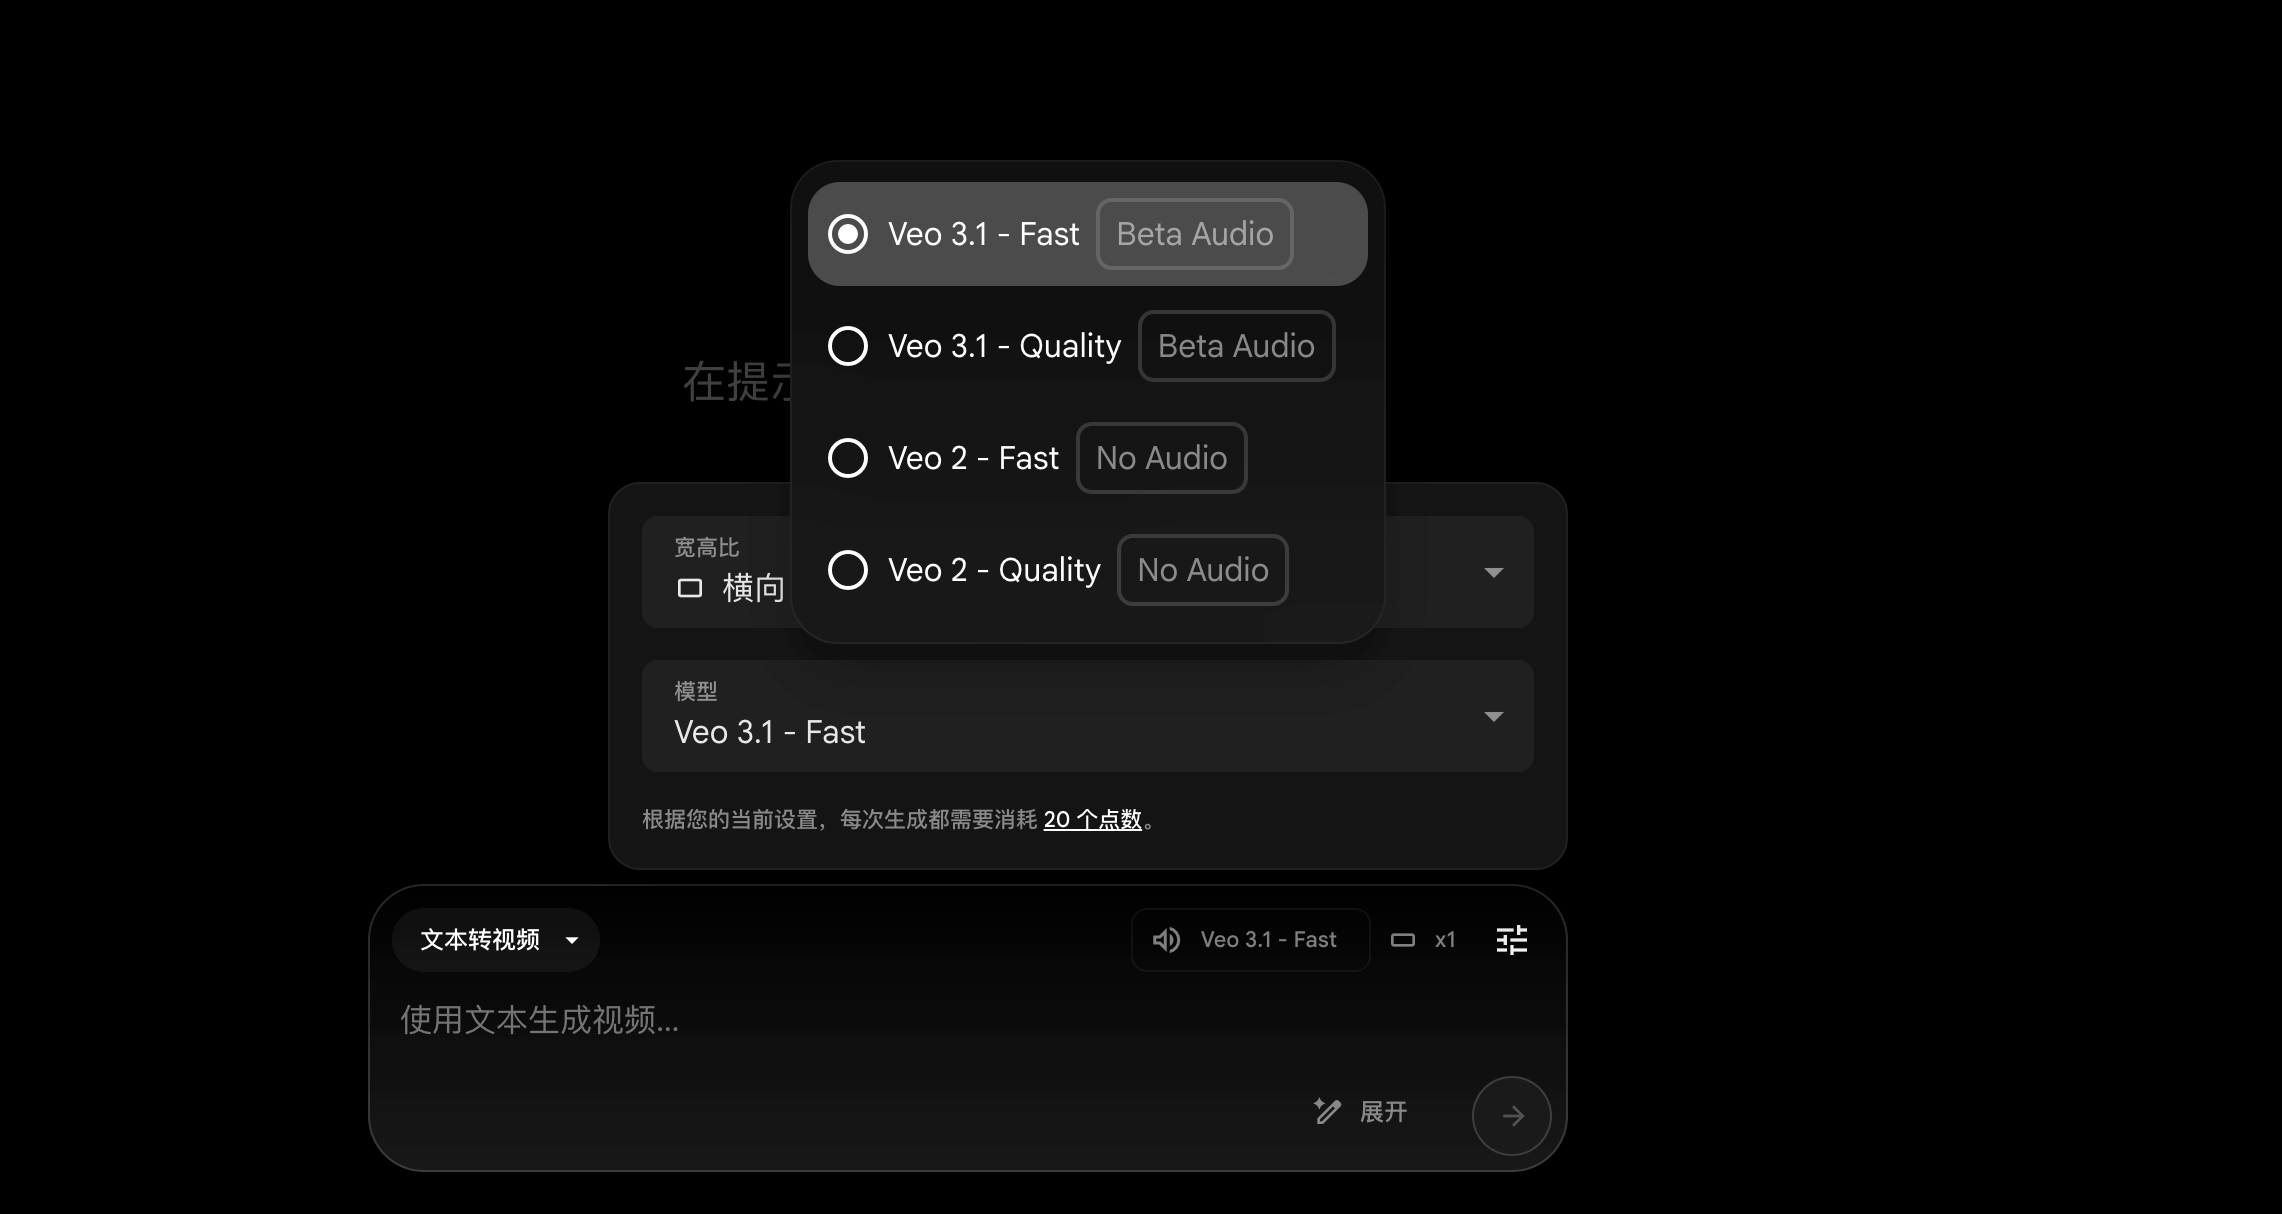
\includegraphics[height=\figheight]{Fig2-7.png}
\caption{Flow model selection dropdown showing available Veo versions. Users can choose between Veo 3.1 - Fast (with Beta Audio) for rapid iteration, Veo 3.1 - Quality for higher fidelity output, or legacy Veo 2 variants. The credit cost per generation is displayed below the model selector. \\ \authorillustration}
\label{fig:flow-model-selection}
\index{figure!Flow model selection}
\end{figure}

\begin{Prompt}
\textbf{Flow/Scenebuilder Configuration Tips}:
\begin{itemize}
\item \textbf{For Speed}: Use ``Veo 3.1 - Fast'' for rapid iteration
\item \textbf{For Quality}: Switch to ``Veo 3.1 - Quality'' for final renders
\item \textbf{Credit Management}: Monitor credit usage; complex Prompts may consume more
\item \textbf{Audio Features}: Beta Audio is only available on Veo 3.1 variants
\end{itemize}
\end{Prompt}

\subsection{Veo 3 vs Sora 2: When to Use Which}
\index{platform comparison}

\begin{table}[H]
\centering
\caption{Platform Selection Guide}
\label{tab:veo-sora-selection}
\begin{tabular}{p{4cm}p{5cm}p{5cm}}
\toprule
\textbf{Use Case} & \textbf{Recommended Platform} & \textbf{Reason} \\
\midrule
Native audio/dialogue & Veo 3.1 & Built-in audio synthesis \\
Character consistency & Sora 2 (Cameo) & Dedicated face/voice system \\
Photorealistic humans & Veo 3.1 & Superior facial rendering \\
Extended duration (60--90s) & Sora 2 Pro & Longer clip support \\
Quick experiments & Gemini + Veo 3 & Conversational interface \\
Precise control & Sora 2 Web or Flow & Detailed parameter panels \\
\bottomrule
\end{tabular}
\end{table}

\section{How to Access NanoBanana Pro}
\label{sec:accessing-nanobanana}
\index{NanoBanana Pro!access methods}
\index{image generation!NanoBanana Pro}

While Sora 2 and Veo 3 handle video generation, many advanced techniques in this book—particularly the Time Travel Selfie workflow covered in Chapter~\ref{ch:time-travel-selfie}—require high-quality \textbf{identity-preserving image generation}. NanoBanana Pro is currently the leading tool for this purpose, excelling at maintaining facial consistency while placing subjects into new environments.

\subsection{Primary Access: Google Gemini Advanced}
\index{NanoBanana Pro!Gemini Advanced}

NanoBanana Pro is available through \textbf{Google Gemini Advanced} subscription. To access:

\begin{enumerate}
\item Navigate to \url{https://gemini.google.com/}
\item Ensure you have an active \textbf{Google One AI Premium} subscription (\$19.99/month as of late 2025)
\item In the Gemini chat interface, NanoBanana Pro capabilities are automatically available for image generation tasks
\item Upload a reference photo and describe the desired scene—Gemini will invoke NanoBanana Pro for identity-locked generation
\end{enumerate}

\begin{Prompt}
\textbf{Sample NanoBanana Pro Request in Gemini:}

``Using the attached photo as reference, generate an image of this person standing in the rain-soaked streets of Blade Runner (1982). Maintain exact facial features. Match the film's neon lighting, cyan and orange color palette, and anamorphic lens characteristics.''
\end{Prompt}

\subsection{Key Capabilities}
\index{NanoBanana Pro!capabilities}

NanoBanana Pro's standout features for creative workflows include:

\begin{itemize}
\item \textbf{Identity Locking}: Maintains facial structure, skin texture, and distinctive features across generated images
\item \textbf{Style Adaptation}: Seamlessly matches reference photo subjects to different lighting conditions, color grades, and visual styles
\item \textbf{Multi-Reference Support}: Can accept both identity reference (your photo) and scene reference (movie still) simultaneously
\item \textbf{High Resolution Output}: Generates images suitable for video upscaling and professional workflows
\end{itemize}

\begin{center}
\fbox{\parbox{0.9\textwidth}{
\textbf{Pro Tip}: If you have access to \textbf{Google Antigravity} (the experimental AI coding environment), you can generate NanoBanana Pro assets directly within your development workflow using the built-in NanoBanana agent. This enables programmatic batch generation for multi-scene projects.
}}
\end{center}

\section*{Chapter Summary}

Key actionable insights for Sora 2 and Veo 3 setup and interface mastery:

\begin{itemize}
\item \textbf{Sora 2 Access}: Web interface at \url{https://sora.chatgpt.com/}, iOS app, or API integration
\item \textbf{Veo 3 Access}: Google Gemini (conversational) or Flow/Scenebuilder (professional)
\item \textbf{System Requirements}: Ensure 16GB+ RAM and stable network connection for optimal performance
\item \textbf{Interface Navigation}: Master the core areas: Prompt input, parameter panel, preview area, and version management
\item \textbf{Platform Selection}: Choose Veo 3 for native audio; choose Sora 2 for Cameo and longer durations
\item \textbf{Progressive Learning}: Begin with basic commands and gradually explore advanced features as confidence builds
\end{itemize}

\section*{Practical Exercises}
\index{practical exercises}

\begin{quote}
\textit{\textbf{Timeless Principle:} Even as interfaces evolve and platforms update, the underlying visual logic---light, composition, rhythm, and emotional resonance---remains eternal. Master these fundamentals, and you will adapt effortlessly to any future tool.}
\end{quote}

\subsection*{Exercise 1: Sora 2 Platform Setup and Optimization}
\textbf{Objective}: Establish optimal working environment for Sora 2 creation.

\textbf{Setup Checklist}:
\begin{enumerate}
\item Test network speed: Ensure 50+ Mbps download for smooth video generation
\item Configure browser: Enable hardware acceleration, clear cache, disable ad blockers for Sora 2 domain
\item Organize workspace: Create dedicated folders for projects, exports, and Prompt libraries
\item Test device performance: Run a simple 10-second generation to verify system capabilities
\end{enumerate}

\subsection*{Exercise 2: Sora 2 Interface Familiarization}
\textbf{Objective}: Master the Sora 2 interface for efficient workflow.

\textbf{Navigation Tasks}:
\begin{itemize}
\item Locate and test each parameter slider (duration, aspect ratio, quality)
\item Practice switching between different view modes (grid, timeline, full-screen)
\item Create and organize your first project folder
\item Export a test generation in multiple formats (MP4, MOV, GIF)
\end{itemize}

\subsection*{Exercise 3: Veo 3 Access via Gemini}
\textbf{Objective}: Successfully access and generate your first video using Veo 3 through Google Gemini.

\textbf{Step-by-Step Tasks}:
\begin{enumerate}
\item Navigate to \url{https://gemini.google.com/} and sign in with your Google account
\item Click the ``Tools'' button and select ``Create videos (Veo 3.1)''
\item Enter a simple Prompt: ``A cat walking across a sunny windowsill, soft morning light''
\item Wait for generation and evaluate the result for quality and Prompt adherence
\item Try the same Prompt with additional detail and compare outputs
\end{enumerate}

\subsection*{Exercise 4: Veo 3 Professional Access via Flow}
\textbf{Objective}: Explore advanced Veo 3 features through Google's Flow/Scenebuilder platform.

\textbf{Exploration Tasks}:
\begin{enumerate}
\item Navigate to \url{https://labs.google/flow} and sign in
\item Select ``Text-to-Video'' from the generation mode menu
\item Click the model selector and compare available options (Veo 3.1 - Fast vs Quality)
\item Generate the same Prompt using both ``Fast'' and ``Quality'' modes
\item Note the differences in generation time, visual quality, and credit consumption
\item Experiment with different aspect ratios (landscape, portrait, square)
\end{enumerate}

\subsection*{Exercise 5: Cross-Platform Comparison}
\textbf{Objective}: Understand the practical differences between Sora 2 and Veo 3.

\textbf{Comparative Analysis}:
\begin{enumerate}
\item Create the same Prompt for both platforms:
\begin{Prompt}
``A person walks through a rainy city street at night, neon signs reflecting on wet pavement, camera follows from behind''
\end{Prompt}
\item Generate on Sora 2 (Web interface) and Veo 3 (Flow with Quality mode)
\item Compare results across these dimensions:
  \begin{itemize}
  \item Visual quality and realism
  \item Motion smoothness and physics accuracy
  \item Audio presence (Veo 3 only)
  \item Generation time and credit/subscription cost
  \end{itemize}
\item Document which platform excels for different aspects of your creative needs
\end{enumerate}
